\nsection{OSN 15 Инструментирование при динамическом анализе: инструментирование исходного кода программ при компиляции, динамическая двоичная трансляция.}

Dynamic analysis can help with some situations when static canno
Динамический анализ может помочь в некоторых ситуациях в которых статический анализ не способен провести анализ
\begin{itemize}
    \item[+] Прочти нет false positives ошибок
    \item[-] Дорогой анализ
    \item[-] Находит ошибки только на конкретном пути исполнения.
\end{itemize}

\textbf{Статическое инструментирование}
Инструментирование — добавление в существующую программу блоков кода, существляющих отслеживание каких-либо её характеристик во время выполнения.

Статическое инструментирование выполняется однократно перед запуском программы.
Статическое инструментирование может выполняться:
\begin{itemize}
    \item на уровне исходного кода — вручную или автоматически;
    \item на уровне бинарного кода — вручную или автоматически.
\end{itemize}

<<Print-debugging>> — пример выполненного вручную статического инструментирования на уровне исходного кода с целью отладки программы.

\textbf{Динамическое инструментирование бинарного кода (DBI)} — разновидность инструментирования бинарного кода, выполняемого во время работы программы. Динамическое инструментирование бинарного кода родственно JIT-компиляции, т.к. предполагает построение выполняющегося кода «на лету».

DBI технология нашла широкое применение от поиска уязвимостей в коде до анализа производительности отдельных участков кода. Одним из простых примеров использования DBI можно считать перехват вызова \textbf{отдельных функций}(PIN). Иногда он используется для подмены значений параметров целевой функции, а иногда просто для замера времени выполнения этой самой функции.

\textbf{Блок трансляции} — не обязательно базовый блок, м.б. более крупные единицы с несколькими выходами.

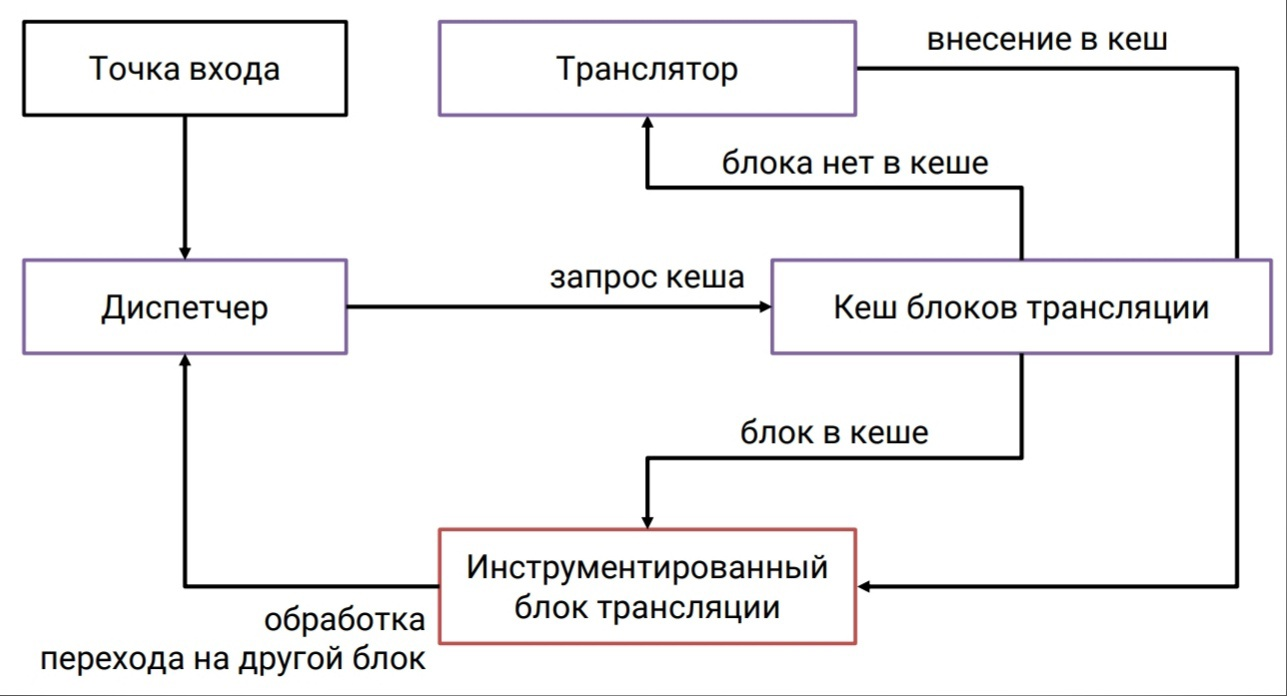
\includegraphics[scale=0.2]{pics/dinamic.png}

Подходы к выполнению инструментированию блока трансляции:
\begin{itemize}
    \item копирование и аннотирование (C\&A — copy-and-annotate); PIN
    \item <<дизассемблирование>> и ресинтезирование (D\&R: disassembleand-resynthesize). Valgrind
\end{itemize}